\chapter{Experiments}
\label{chapter:experiments}
% \todo{for motivation, maybe consider the introduction \href{https://arxiv.org/pdf/1712.03346.pdf}{here}}

In the introduction (section \ref{chapter:introduction}) we asked what a good protein representation is, what the advantages and disadvantages of global versus local representations are, and how the properties of the representation affect the performance on downstream tasks.

In order to find answers, we have carried out a number of experiments, applied to each model. There are broadly two experimental settings: (1) mutation effect prediction and (2) tasks assessing protein embeddings \cite{rao2019evaluating}. The first setting evaluates the mutation effect prediction of the models, based on the learned distribution over proteins. This is of interest, as mutation effect prediction is tightly connected to the underlying evolutionary generating process, and what properties the mutated protein possesses. The second setting is a benchmark assessment of the performance of the protein representations on downstream tasks.

In this chapter we report how we did it and what the results were. In section \ref{sec:experimental_setup} the experimental settings are accounted for, including commonalities between the experiments such as what language framework we used to implement the models, and hardware used for training and testing. 

There are 3 conceptually different model architectures that we have tested. Each model architecture is described in chapter \ref{chapter:models} and has its own section here. 

% In section \ref{sec:unirep_experiment}, the UniRep model \cite{alley2019unified}. UniRep is a recurrent model, and can thus handle variable-length sequences, and can thus be trained on global protein databases. We explore the performance of a variant of the UniRep model on downstream tasks.

% In section \ref{sec:variational_autoencoders_experiement}, we explore the usefulness of the Variational Autoencoder on protein sequences. Specifically, we train a Variational Autoencoder model on sequences within single protein families, obtaining a separate model for each family. The Variational Autoencoder does not handle variable-length sequences though, so each family of proteins must be aligned to a single length.


% \todo{introduce other approaches, i.e. WaveNet, transformer etc.}

\section{Experimental Setup}
\label{sec:experimental_setup}
For all of our experiments, we utilized PyTorch \cite{NEURIPS2019_9015}, a modern machine learning framework. PyTorch provides, among other things, automatic gradient computation, optimized modules of frequently used modeling architectures and low-level GPU integration for efficient training. These are fundamental dependencies in our modeling methods that has allowed a much faster development process. We preferred PyTorch over its alternatives due to its flexible yet concise usage.

In the mutation effect prediction setting, we train each model on 80\% of the sequences, using the rest for validation, usually with 128 batch size (in some cases a smaller batch size is used due to memory constraints). Training continues until we see no improvement on the validation score, and keep the model that performed best on the validation set. In terms of hardware, we used a cluster of NVIDIA RTX 2080 graphics cards to perform both training and testing. In most settings, a single GPU is used, which contains 24 GB RAM. Pretraining of the WaveNet model was done on 4 such GPUs in parallel, in order to train faster.

\subsection{Mutation Effect Prediction}
\label{sec:mutation_effect_prediction}

% There are many possible metrics one could use to compare our experiments 
% \todo{motivate why we are measuring what we do}. We decided to evaluate our models by examining their ability to predict the effect of mutations in proteins. 

The models have in common that they all produce a distribution over proteins $\px$, each in their own way. The interpretation of $\px$ is that it is the probability of the protein sequence $\ve{x}$ being generated by the evolutionary process. This probability allows for an informed comparison of protein in terms of how likely they are to exist; if the probability of one protein is higher than another, then the first should be expected to have higher measures of properties related to persistence, such as stability and other functional constraints. Specifically, it allows for the comparison of some protein with its mutations; if a mutation of a protein increases its probability, then this increase is likely to be associated with an increase in favorable properties of the protein due to the mutation. This is called \textit{mutation effect prediction}, and it has been shown that the metric
\[\log \frac{p(\ve{x}_{\text{wild-type}})}{p(\ve{x}_{\text{mutant}})} = \log p(\ve{x}_{\text{wild-type}}) - \log p(\ve{x}_{\text{mutant}})\]
correlates with many different effect predictions of proteins \cite{hopf2017mutation}. Here, $\ve{x}_{\text{wild-type}}$ is a wild-type protein, i.e. as it occurs in nature, and $\ve{x}_{\text{mutant}}$ is a mutated version of the same protein. This ratio can be produced by the trained models, and is what we use to calculate correlation with experimental data. The intuition behind the metric is that a higher ratio (above 0) means that the mutation was beneficial for the protein, as it is now more likely than the wild-type, while a negative ratio means that the mutation is likely to be detrimental. Predicting the effect of protein mutations is a relevant task, because examination of mutations is how protein engineering is often performed (such as optimizing a known protein by examining its mutations).

The final outcome in this experimental setting is thus a correlation coefficient $\rho \in [-1, 1]$, in our case the Spearman's $\rho$ coefficient, which in short is a nonlinear dependency measure between two datasets. In short, how well can you fit a monotonically increasing function to describe the datasets; this is more general correlation than Pearson correlation, which fits a linear function. The more correlation deviates from zero, the more the model predictions comply with experiments, which is desirable.

\subsubsection{Data}
\label{sec:data}
The data used for training the various models presented in this thesis is invariably derived from the Universal Protein Resource database (UniProt) \cite{uniprot2007universal}; protein families and alignments are curated as specified in \cite{riesselman2018deep}: the UniRef100 protein dataset is iteratively traversed with the 
\textsc{jackhmmer} protein analysis search tool \cite{eddy1992hmmer} for a given query protein.

% protein family source: https://www.ebi.ac.uk/training/online/course/introduction-protein-classification-ebi/protein-classification/what-are-protein-families
A protein family is a set of proteins that share functionality or structure across organisms because of a shared evolutionary history. In the complex process of protein generation it is, simply put, genes that determine the protein outcome. If proteins share a gene ancestor, we say that the proteins are \textit{homologous} and assumes this is the case when the proteins share similar structure and function. Families induce a hierarchical structure onto protein space, collecting proteins into groups and subgroups that share a common protein ancestor. Determining this hierarchy is nontrivial and usually require probabilistic models to uncover. Protein families can be decided using \textit{profile hidden markov models} (HMM's). These models captures changes between a set of similar proteins, i.e. deletions and insertions of amino acids by casting the changes into transitions and states in a Markov model with associated probabilities for each transition \cite{eddy1998profile}. This model is the called the profile and can be used to iteratively search a given protein database for similar proteins. These can then be included in the family if their similarity if above some threshold. A new profile can then be modelled based on the new set of proteins. This can be repeated a fixed number of iterations, or until no new proteins are added to the collection (i.e. the search has converged on a set of proteins). This procedure is what the \textsc{jackhmmer} search tool accomplishes.

The protein family datasets we have used are the sequence alignments, and their associated experimental data, made available by \cite{riesselman2018deep}. We have chosen a subset of 5 families to assert the diversity of the models: 
\begin{itemize}
    \item E.coli $\beta$-lactamase (BLAT ECOLX)
    \item Human Calmodulin-1 (CALM1 HUMAN)
    \item Yeast regulatory protein GAL4 (GAL4)
    \item Yeast ATP-dependent molecular chaperone HSP82 (HSP82)
    \item Human GTPase HRas (RASH HUMAN).
\end{itemize}
The protein families are chosen on the basis of the expected performance on the sets, based on the results achieved in \cite{riesselman2018deep}: We have tried to select families the captures variance in the performance of the models, i.e. we want families that are both easy and difficult for the models to predict, and in between. Table \ref{tab:datasets} below displays some metadata of the datasets.

\begin{table}[ht]
    \centering
    \begin{tabularx}{\textwidth}{l rrrrr}
    \hline
    & \textbf{BLAT ECOLX} & \textbf{CALM1 HUMAN} & \textbf{GAL4} & \textbf{HSP82} & \textbf{RASH HUMAN} \\ \hline
    \textbf{Family Size}    & 8403 & 36224 & 22985 & 23447 & 84762 \\
    \textbf{Effective Size} & 2225 &  4754 &  3542 &  1321 &  5954 \\
    \textbf{\# Mutations}   & 4788 &  1868 &  1104 &  4313 &  3078 \\
    \textbf{Alignment Size} &  263 &   149 &    75 &   240 &   189 \\
    \hline
    \end{tabularx}
    \caption{Datasets used for for each protein family.}
    \label{tab:datasets}
\end{table}

\paragraph{Sample weights} A protein family dataset consists of protein sequences that share a common ancestor. However, such datasets are not guaranteed to be evenly distributed among sequences from descendants. For this reason, some protein sequences might be overly represented, while others might not. In order to balance the dataset, protein sequences have be reweighted such that similar samples are grouped together and weight in inverse proportion to the size of the group. For a specific protein family with $n$ protein sequences $p_1, p_2, \ldots, p_n$, this leads to an effective number of samples, $n_{\texttt{eff}} = \sum_{i = 1}^n \pi_i$, where
    \[ \pi_i =\prts{\sum_{j = 1}^n \brts{ \text{ $p_i$ is similar to $p_j$ } }}^{-1}. \]
Brackets denote the indicator function of the statement inside the brackets. We follow the steps of \cite{riesselman2018deep} and \cite{hopf2017mutation} and measure similarity by normalized Hamming distance, with a threshold of 0.2, meaning that if two sequences share at least 80\% of their positions, they are similar:
  \[ \brts{ \text{ $p_i$ is similar to $p_j$ } } = \brts{ \ \texttt{hamming}\prts{p_i, p_j} \leq 0.2 \ }.\]
The effective dataset sizes are shown in table \ref{tab:datasets} in the effective size row.
\paragraph{Experimental data} used to correlate our predictions are not necessarily the same metric across protein families, but each experiment measure levels of various fitness-related properties for a single mutation. E.g. the experimental results for $\beta$-lactamase is derived from \cite{stiffler2015evolvability} and is, to our best understanding as computer scientists, a study of fitness effects of single  amino acid mutations by observing growth in E. coli cells under 2500 $\mu$g/ml ampicillin. 

% \todo{is data i.i.d ? is this an assumption we make? I guess we assume that the data distribution is fixed and that data samples are identically distributed. But are we assuming independent sampling, and if so, is this a valid assumption?}

% from https://cryptogenomicon.org/2012/04/16/interactive-iterative-searches-using-jackhmmer/
% Jackhmmer is the iterative search method in the HMMER package, analogous to PSI-BLAST.  A typical jackhmmer search starts with a single protein sequence.  This sequence is searched against a target protein sequence database (such as UniProt or NR) by converting the sequence to a profile hidden Markov model (HMM), using a substitution matrix and affine gap penalties.  The target sequences that score above the inclusion threshold from this first search are then aligned and used to construct a second profile HMM.  In this and subsequent iterations, the conservation pattern specific to this alignment is used to determine the probabilities of seeing different amino acids, a deletion or an insertion at each position in the profile HMM.  This second profile HMM is then searched against the same target database and will typically find more distant homologs to the original query sequence.  These new results can then be aligned as before and used to initiate another search (or iteration) and so on.  Sometimes, no additional sequences can be found between iterations and the search is deemed to have converged.

\subsection{TAPE}
\label{sec:tape}
Unlike the variational auto-encoder, the UniRep and WaveNet models do not include a compact representation in their training, since they are inherently sequence-to-sequence models, while the variational auto-encoder is a bottleneck model. As discussed in section \ref{sec:seq2seqvsbottleneck}, a compact representation can however be extracted from a sequence-to-sequence model, after training has been completed. Judging the usefulness of these representations cannot be done by the training or validation procedure, since it is not part of the model's training process. Hence, the representations must be evaluated externally.

In order to assess the quality of these representations, we turn to a standard set of downstream tasks associated with protein representation learning -- these are the \textit{Tasks Assessing Protein Embeddings}, otherwise known as TAPE \cite{tape2019}. TAPE includes a diverse set of protein-related tasks that are considered to be useful for a protein representation. Using TAPE, we can quantitatively compare the representations of UniRep and WaveNet to each other, as well as to the benchmarks already provided by TAPE on other models.

Because the TAPE tasks are so diverse, they can show if a model's representation is generally useful, or reveal the strengths and weaknesses of different models, which may inform an application on which model is the most suitable to use for a given problem.

Aside from the definition of the tasks themselves, TAPE also provides a general training framework which makes it easy to adapt an existing model to the TAPE task evaluation process. This framework also provides general top models, which are used in the training for each task. By using the same top model on all the different models evaluated, TAPE provides a fair ``competition''.

Concretely, TAPE consists of the following 5 tasks:
\begin{description}
    \item[Secondary Structure Prediction:] This task involves classification of secondary structure (see section \ref{sec:protein_structure}) for each of the amino acids of the input sequence. The resulting score is an accuracy on the three classes ``Helix'', ``Strand'' and ``Other''. Secondary structure prediction is a useful first step to figuring out the function of a protein. Data is provided by \cite{pdb, casp, netsurfp}.
    \item[Contact Prediction:] In this task, the model must predict whether a pair of amino acids in a protein are in contact ($<$ 8Å distance) or not. The resulting score is hence an accuracy on two classes. This information is highly useful when analyzing the dependencies between the amino acids, or when trying to figure out the tertiary structure. Data is provided by \cite{scop, casp, proteinnet, pdb}.
    \item[Remote Homology Detection:] This task asks the model to predict the protein fold of an input sequence. The score is an accuracy on the 1195 possible folds. Data is provided by \cite{scop}.
    \item[Fluorescence:] In this task, the model must predict the fluorescence of the input protein. This can be useful when trying to optimize a protein's function by introducing mutations. This is a regression task, hence the score is given as a Spearman correlation. Data is provided by \cite{sarkisyan2016}.
    \item[Stability:] The final task asks the model to predict the stability of the input protein. Stability is a highly desirable property, as a protein must be stable for long enough for its purpose to be fulfilled. Predicting stability is therefore very useful. Like the previous task, this is a regression problem and the score is thus given as a Spearman correlation. Data is provided by \cite{rocklin2017}.
\end{description}

Of the 5 tasks above, 

\section{UniRep}
\label{sec:unirep_experiment}
As described in section \ref{sec:unirep_model}, the choice of RNN and hidden state size of the UniRep model is not very significant. In accordance with this, we decided not to use the canonical UniRep model and instead opted to use an LSTM with a 512 hidden state size, without truncated backpropogation. Our previous work on UniRep suggests that the difference between the canonical UniRep model and this variant should be insignificant \cite{unirepproject}. At the same time, our model is smaller and can make use of PyTorch's inbuilt LSTM module, both of which contribute to a much more computationally cheap model.

We train UniRep in two ways; with and without global pre-training. When using pre-training, we first train an UniRep model on the UniRef50 dataset of sequences, which contains roughly 39 million protein sequences at the time of writing. This gives the model a chance to learn general protein properties from the global protein space.

When evaluating for individual tasks, we finetune the model (which may or may not have been pretrained) for the specific task at hand. For the mutation effect prediction task, this involves training a model for each protein family. For the TAPE tasks, one model is trained in TAPE's training framework for each task. We also evaluate UniRep on the tasks using only the pretraining. This results in three configurations for the tasks: Pretrained, Finetuned and Pretrained + Finetuned.

\subsection{Results}
\subsubsection{Mutation Effect Prediction}
We evaluate UniRep on the mutation effect prediction task by feeding the sequences through UniRep's entire architecture, as illustrated in figure \ref{fig:unirep_architecture}. This gives us a log-probability for each amino acid, given the sequence up to that point. We obtain the log-probability for the entire sequence by summing the log-probabilities of the amino acids.

Table \ref{tab:unirep_mutation_results} shows UniRep's performance on the mutation effect prediction task.

\begin{table}[ht]
    \centering
    \begin{tabularx}{\textwidth}{lrrrrr}
    \hline
    & \textbf{BLAT ECOLX} & \textbf{CALM1 HUMAN} & \textbf{GAL4} & \textbf{HSP82} & \textbf{RASH HUMAN} \\ \hline
    \textbf{Finetune}            & 0.4390          & 0.2611          & \textbf{0.4570} & \textbf{0.3839} & 0.2825 \\
    \textbf{Pretrain + Finetune} & \textbf{0.4432} & \textbf{0.2891} & 0.3658          & 0.3757          & \textbf{0.2963} \\
    \hline
    \end{tabularx}
    \caption{Mutation effect prediction correlation for the UniRep model, with and without pretraining. Each measure is an average over five runs.}
    \label{tab:unirep_mutation_results}
\end{table}

\subsubsection{TAPE}


\subsection{Discussion}
\todo{argue why hyperparameters are sufficient}
\todo{discuss why the local performance is poor}
\todo{discuss model relevance for protein representation}

\section{VAE}
\label{sec:variational_autoencoders_experiement}

We trained one model for each protein family we examined, but kept the architecture of the model constant throughout. The training process uses both the encoder and the decoder. The encoder compressed the sequence from its original size (that is, a flattened one-hot encoding) into two 1500-dimensional layers, before reaching the 30-dimensional probabilistic bottleneck representation. Samples are drawn from the representation, which are sent into the decoder, which has a 100-dimensional layer, followed by a 2000-dimensional layer, before reaching the original sequence size again. The architecture is illustrated in figure \ref{fig:vae_architecture}.

\begin{figure}[ht]
    \centering
    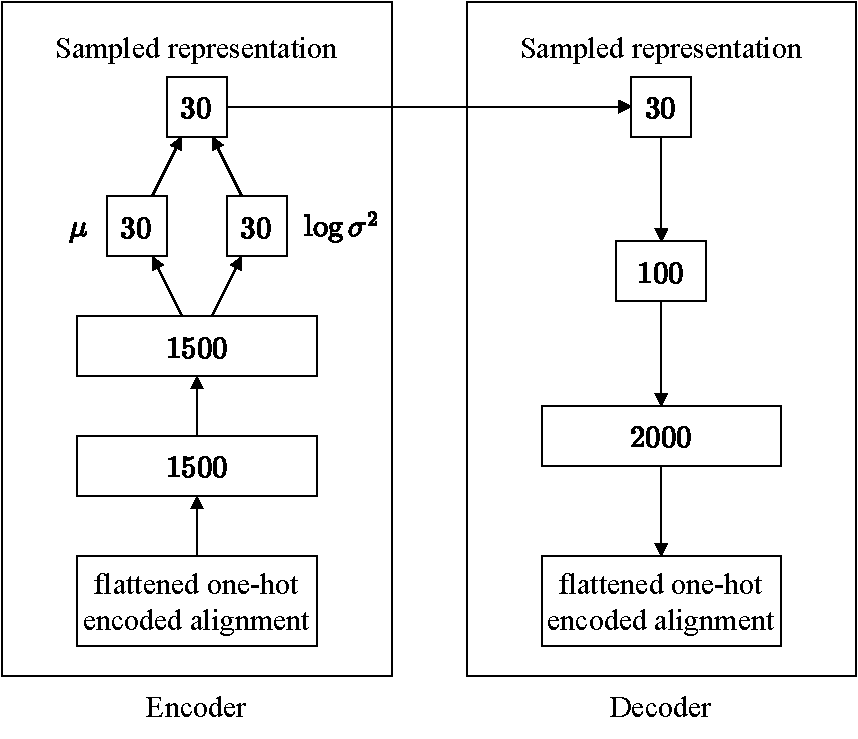
\includegraphics{report/figures/VAE_architecture.pdf}
    \caption{Architecture of the VAE model.}
    \label{fig:vae_architecture}
\end{figure}

\subsection{Results}
When evaluating the model, we are primarily interested in the usefulness of the representations produced by the encoder. Thus, the decoder is only used for training the encoder, or for recovering the protein sequence from the representation given by the encoder. We evaluate the representation by examining its properties, as well as using it for a predictive downstream task.

Figure \ref{fig:2dimvae} shows the mean of the representations of proteins from the $\beta$-lactamase protein family, colored by phylum, as produced by a VAE model of the same dimension as described earlier, except with a 2-dimensional bottleneck size, so that we can plot the representation. The structure of the representations resemble that of a phylogenetic tree, suggesting that the model correctly identifies the evolutionary similarities between the different variants of $\beta$-lactamase. A similar phylogenetic tree-like structure is seen when using the model on other protein families.

\begin{figure}[ht]
    \centering
    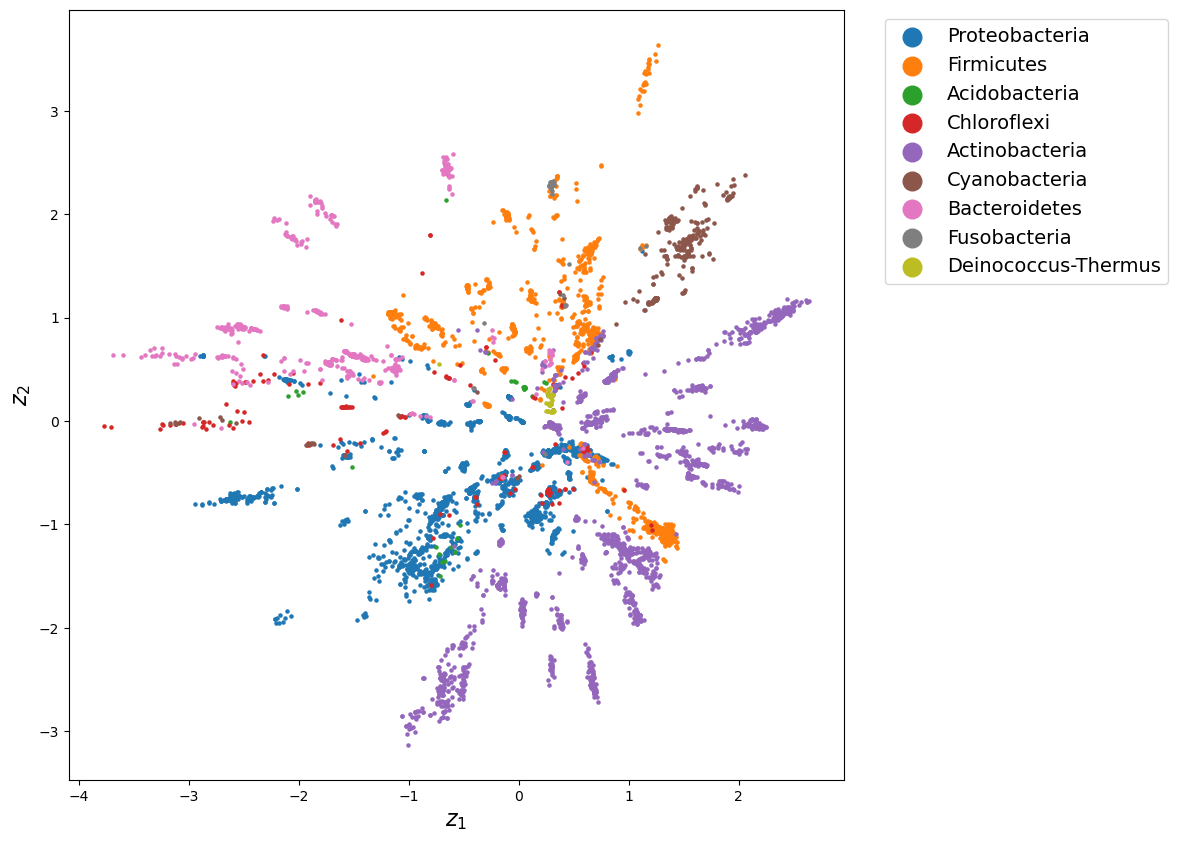
\includegraphics[width = \linewidth]{report/figures/vae_representation2d.png}
    \caption{Mean of the protein representations of selected phylums of $\beta$-lactamase, produced by a VAE model with a bottleneck layer size of 2.\todo{update figure}}
    \label{fig:2dimvae}
\end{figure}

\todo{Show concrete example on how a protein sequence is encoded and its decoded reconstruction. Maybe as a figure and color-code the wrong residues. Discuss reconstruction accuracy (which is $\approx$ 60\% I think)}

\todo{show loss plots during training. use as argument for e.g. model is not overfitting, or model has learned what it can or something along those lines}

\todo{show spearman $\rho$ during training. discuss: are we biasing our results by looking at spearman during training?}

\todo{show explained variance figure. discuss: why is basically all variance explained by < 15 dimensions? can we really explain all variance of a protein family in 15 features or less?}

\todo{show figure of results on ALL protein family datasets. maybe discuss any performance variation. if possible, conclude that the model framework seems to work across many protein families/datasets.}

\begin{table}[ht]
    \centering
    \begin{tabularx}{\textwidth}{lrrrrr}
    \hline
    & \textbf{BLAT ECOLX} & \textbf{CALM1 HUMAN} & \textbf{GAL4} & \textbf{HSP82} & \textbf{RASH HUMAN} \\ \hline
    \textbf{MAP}                 & 0.5685 & 0.2789 & 0.3916 & 0.4734 & 0.4870 \\
    \textbf{MAP + sparsity}      & 0.6550 & \textbf{0.2866} & \textbf{0.4700} & 0.4875 & 0.4704 \\
    \textbf{Bayesian}            & 0.6878 & 0.2732 & 0.3658 & 0.4653 & \textbf{0.5003} \\
    \textbf{Bayesian + sparsity} & \textbf{0.7124} & 0.2733 & 0.3664 & \textbf{0.5130} & 0.3762 \\
    \hline
    \end{tabularx}
    \caption{Mutation effect prediction correlation using variants of the VAE model. Each measure is averaged over five sessions.}
    \label{tab:vae_results}
\end{table}

\todo{show the latent space of the BLAT ECOL query protein and the latent space representations of all its mutations - it should show that the mutations are local to the query representation in latent space. discuss that this indicates that distance in latent space is connected to protein similarity.}

\todo{show softmax distribution figure of some example proteins. discuss what we are seeing; is the model very certain of a few amino acids, or does it distribute probability more evenly?}

\todo{maybe do linear interpolation between two proteins in latent space? to show that euclidean distance measure is inadequate - future work etc.}

\todo{t-SNE of 30-latent space variables. free real estate}

\subsection{Discussion}

\section{WaveNet}
\label{sec:wavenet_experiment}
The WaveNet model architecture was trained on the protein family datasets (see section \ref{sec:data}) for mutation effect prediction. The experiments are conducted by training the model to reconstruct sequence inputs, compelling the model to learn factors that drive protein characteristics. For a given input sequence, the model predicts each residue position based on the sequence observed so far at that position. We trained a total of 6 models: 3 observing sequences in a ``forward'' direction, and 3 observing sequences in a ``backward'' direction. This ensemble determine the mutation effect predictions. We have adopted hyperparameter settings as described in \cite{riesselman2019accelerating}, using L2 regularization of model parameters with coefficient $\lambda = 1$, a clipping of gradient norms to 100, and an aggressive dropout probability of $\sfrac{1}{2}$ on model components. The WaveNet architecture was instantiated with a dilation stack of 6 dilation blocks, each consisting of 9 dilation layers (that is, dilation in the range $1, 2, 4, \ldots, 256$). \todo{should the range be larger? what about sequences that are longer than 256} The number of channels used in the Norm Conv layers is 48 (with the exception of final and initial convolutions which map to and from the number of candidate residues).

In the case study of the $\beta$-lactamase protein family, we have two variants of the experiment: one where each protein sequence input is equally weighted in the loss calculation, and one with sequence weights according to sequence similarity (see \ref{sec:data} for details).

\subsection{Results}

\subsubsection{Mutation Effect Prediction on $\ve{\beta}$-Lactamase Protein Family}
Each model in the ensemble of 6 models was trained using the ADAM optimizer \cite{kingma2014adam} with standard parameters, specifically a learning rate of $0.001$. \todo{discuss why learning rate is immensely important; shifting the lr a little bit basically means the models learn almost nothing} 

 If the training loss of the model did not improve at least every other epoch, we stopped the training procedure. We used a batch size of 128 and used $20\%$ of the data samples as a validation set.

The stopping criteria resulted in relatively short training sessions of less than 20 epochs. In the unweighted case, it is significant for performance to keep a low patience. This behavior is discussed further in \ref{sec:wavenet_discussion}. %The correlation coefficient $\rho$ between predictions and measured experiments steadily increase during training as seen in figure~\ref{fig:wn_f2_rho}~and~\ref{fig:wn_b2_rho}.

% \todo{should this even be here?}

% \begin{minipage}{\linewidth}
% 	\centering
% 	\begin{minipage}{0.49\linewidth}
% 		\begin{figure}[H]
% 			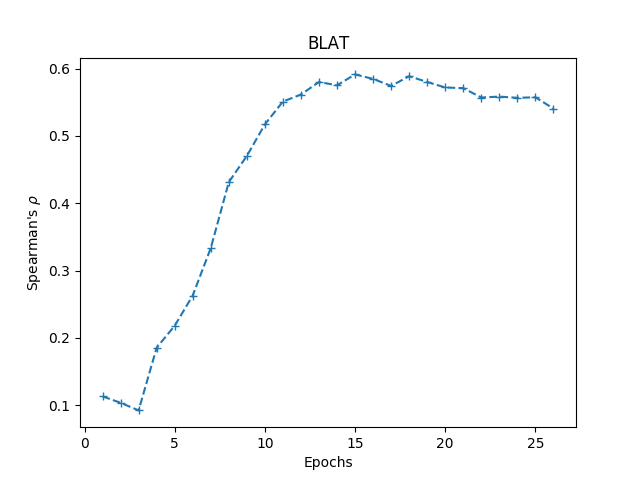
\includegraphics[width=\linewidth]{report/figures/wn_f2_rho.png}
% 			\caption{Forward-pass training correlation.}
% 		    \label{fig:wn_f2_rho}
% 		\end{figure}
% 	\end{minipage}
% 	\hfill
% 	\begin{minipage}{0.49\linewidth}
% 		\begin{figure}[H]
% 			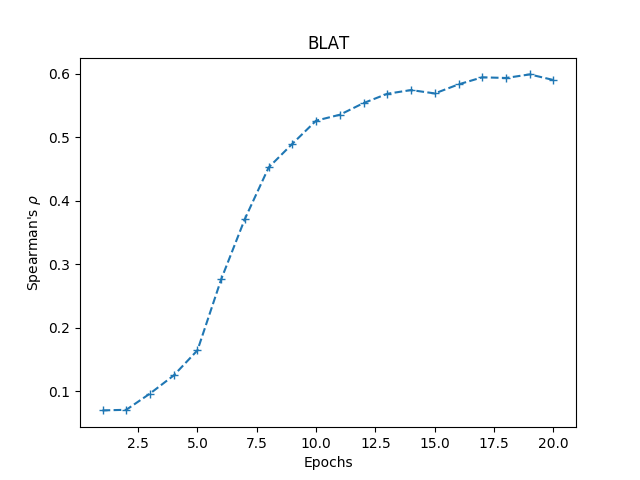
\includegraphics[width=\linewidth]{report/figures/wn_b2_rho.png}
% 		    \caption{Backward-pass training correlation.}
% 		    \label{fig:wn_b2_rho}
% 		\end{figure}
% 	\end{minipage}
% \end{minipage}

% For the unweighted models, the model mutation effect predictions have a Spearman $\rho$ correlation with experimental results of 0.627. For the weighted models, the mutation effect predictions have a correlation of 0.717. This indicates that sample weights provide a significant performance addition. This is discussed further in section \ref{sec:wavenet_discussion}.

\begin{table}[ht]
    \centering
    \begin{tabularx}{\textwidth}{l ccccc}
    \hline
    & \textbf{BLAT ECOLX} & \textbf{CALM1 HUMAN} & \textbf{GAL4} & \textbf{HSP82} & \textbf{RASH HUMAN} \\ \hline
    \textbf{No pretraining} & 0.613 & 0.287 & 0.54 & 0.51 & 0.432 \\
    \textbf{Pretraining}    & & & & & \\
    \hline
    \end{tabularx}
    \caption{Mutation effect prediction Spearman's $\rho$ correlation scores for the WaveNet model on different datasets. With-- and without pretraining.}
    \label{tab:wavenet_rho_results}
\end{table}

\subsubsection{Mutation Effect Prediction on other Protein Families}
\todo{rho figure for all datasets (or the subset data we choose)}

\todo{accuracy}

\todo{show representation}

\todo{TAPE results on wavenet representations}
\subsubsection{WaveNet Representation: TAPE}
\begin{table}[ht]
    \centering
    \begin{tabularx}{0.93\textwidth}{cccccc}
    \hline
    \textbf{Pretrain} & \textbf{Fine-tune} & \textbf{Secondary Structure} & \textbf{Homology} & \textbf{Fluorescence} & \textbf{Stability} \\ \hline
    No  & No  & 0.3901 & 0.0000 & -0.0150 & 0.0800 \\
    No  & Yes & 0.7014 & 0.1879 & 0.3806 & 0.7563 \\
    Yes & No  & & & & \\
    Yes & Yes & & & & \\
    \hline
    \end{tabularx}
    \caption{WaveNet performance on the TAPE tasks. Generated protein representations are with-- and without pretraining and fine-tuning.}
    \label{tab:wavenet_tape_results}
\end{table}

\subsection{Discussion}
\label{sec:wavenet_discussion}
The WaveNet model performs comparatively to current state of the art \todo{really, though?} when sample-weights are applied, confirming that the model has the potential to perform among the current best models on this task. It does however degrade in performance once samples are uniformly weighted, which shows that there is still room for improvement. Because of the significance of weights, finding a weighting scheme that does not rely on an alignment is a reasonable next step. One such approach could be to apply unsupervised clustering algorithms to the dataset and distribute weight inside clusters. This is a common problem associated with the data and not the model, and so we discuss this separately in section \todo{discuss this somewhere, was thinking a discussion section for all models/data maybe?}

Most strikingly, the architecture seem to capture signal from the entire protein sequence by the gradually expanding convolutions, alleviating the need for recurrence in the network, while maintaining performance. This is a desirable property as, in contrast to RNNs, convolutions can be performed in parallel, and so one should expect an improvement in runtime on GPU accelerated training. In addition, this architecture still afford the desirable length-invariant property of the recurrent neural network (as long as all sequences are at most a specified maximum length that can be set sufficiently large to accommodate any practical setting).

In terms of trainable parameters, the WaveNet architecture is also significantly smaller, requiring gradients for about 600,000 parameters. This is a small model in comparison with most attention-based models, usually requiring millions of parameters. The VAE model in our experiments require about 50 million parameters and is thus significantly larger. 

\todo{show what happens if you increase patience on unweighted wavenet}

\todo{discuss model relevance for protein representation}
There are two major drawbacks: The performance loss due to unweighted samples, and the fact that the model produces no explicit, learnable, fixed-length representation for its inputs. The issue of extracting fixed-length representations for variable-length inputs is shared among all three variable-length models (i.e. not the VAE), and so we discuss this separately in section \todo{discuss extraction of representation from wavenet, unirep and transformer, give reference here}.

% \section{Transformer}
% \label{sec:transformer_experiment}

% \todo{fill in values here} In our concrete Transformer model, we embed the amino acids to X-dimensional vectors. We use X number of self-attention heads with X encoder layers and X decoder layers. The linear layers use weights of size X, and we use X\% dropout.

% \subsection{Results}
% \subsection{Discussion}
% \todo{discuss model relevance for protein representation}